%THIS IS AN EXAMPLE OF HOW YOU MIGHT INTRODUCE A CHAPTER WHICH HAS ALREADY BEEN PUBLISHED.
\cleartoevenpage
\pagestyle{empty}	%Use this to suppress the header from the preceding chapter.

\noindent
%The following publication has been incorporated as Chapter~\ref{Chap:label}.

%\noindent
%1.~\cite{citationkey} \textbf{Your Name}, Co-author 1, and Final Author, \href{linktoyourpaper}{Title of your paper}, \textit{Journal} Issue, Number, Year

\begin{table}[h]
	\begin{center}
	\begin{tabular}{|c|l|l|}
		\hline
		Contributor & Statement of contribution & \% \\
		\hline
		\textbf{Your Name}				& writing of text 					& 70\\
															& proof-reading							& 60 \\
															& theoretical derivations 	& 70\\
															& numerical calculations 		& 100\\
															& preparation of figures 		& 80 \\
															& initial concept						& 10 \\
		\hline
		Co-author 1								& writing of text 					& 20\\
															& proof-reading							& 10 \\
															& supervision, guidance 		& 20\\
															& theoretical derivations 	& 10\\
															& preparation of figures 		& 20 \\
															& initial concept						& 10 \\
		\hline
		Final Author							& writing of text 					& 10\\
															& proof-reading							& 30 \\
															& supervision, guidance 		& 80 \\
															& theoretical derivations 	& 20 \\
															& preparation of figures 		& 10 \\
															& initial concept						& 80 \\
		\hline
	\end{tabular}
	\end{center}
\end{table}

%-------------------------------------------------------------------------------------------------------%
%-------------------------------------------------------------------------------------------------------%
%-------------------------------------------------------------------------------------------------------%
%-------------------------------------------------------------------------------------------------------%
%-------------------------------------------------------------------------------------------------------%
%-------------------------------------------------------------------------------------------------------%
%This is an internal chapter of the thesis.
%If you have a long title, you can supply an abbreviated version to print in the Table of Contents using the optional argument to the \chapter command.
\chapter[Process biokinetics of phototrophic systems]{A description of the process biokinetics of phototrophic systems}
\label{Chap:chap2}	%CREATE YOUR OWN LABEL.
\pagestyle{headings}

This chapter is based upon work which has been published during the course of the PhD programme.\\

D. Puyol, \textbf{E. Barry}, T. H\"{u}lsen, and D. Batstone. A mechanistic model for anaerobic phototrophs
in domestic wastewater applications: Photo-anaerobic model (PAnM).
\textit{Water Research}, 116:241–253, 2017. Publisher: Elsevier Ltd.

\section*{Abstract}
Purple phototrophic bacteria (PPB) have been recently proposed as a potential organism for accumulative biotechnologies for wastewater treatment with assimilative removal of nutrients, low greenhouse gas emissions, and a neutral to positive energy balance. PPB have a complex metabolism which can be regulated for process control and optimisation. Since microbial processes governing PPB metabolism differ from traditional processes used for wastewater treatment, a model basis has to be developed to be used a a framework for further detailed modelling under specific situations and environments. This work presents a mixed population phototrophic model for domestic wastewater treatment in anaerobic conditions. The model includes photoheterotrophic, chemoheterotrophic, and photoautotrophic growth, as well as hydrolysis and biomass decay. Photoheterotrophic growth is divided into soluble volatile organic fatty acids with ethanol, and acetate as organic substrates. The main processes have been evaluated through targeted batch experiments, and the key kinetic and stoichiometric parameters have been determined. Parameters were estimated in batch simulations against measured data, and the model was assessed by the simulation of a continuous process.

\section{Introduction}
\label{Sec:chap2_intro}

The treatment of wastewaters is currently seeing a trend away from merely treating wastes to recapturing and reusing the energy and nutrients contained within the streams. Of increasing interest are photosynthetic and phototrophic organisms, such as microalgae \cite{ward2014} and purple phototrophic bacteria (PPB) \cite{hulsen2014} respectively. While both organisms can be used to partition organics and nutrients to a solid phase for reuse, PPB present an advantage in that they are able to recycle electrons during cyclic anoxygenic photosynthesis, meaning they can harvest and retain electrons, resulting in a higher energetic efficiency than that of algae. Maximal photoconversion efficiencies to chemical energy are also higher for PPB at 6-8\% \cite{miyake1987} than for algae at less than 5\% \cite{posten2009}. Despite numerous studies demonstrating use cases of PPB to produce bioplastics \cite{melnicki2009} and treat wastewaters such as different meats, dairy and sugar \cite{hulsen2018}, latex \cite{kantachote2005}, and tofu \cite{zhu1999}, the widespread adoption of practical technologies has been slow. This is in large part due to several process limitations, such as photon conversion efficiency (or energy costs), solid-liquid separation issues for harvesting, and the requirements of extra readily biodegradable chemical oxygen demand (COD) in order to achieve discharge limits in nitrogen and phosphorus \cite{hulsen2015}.
\skippingparagraph
Process modelling can be used to address the aforementioned issues, as well as to better understand and optimise phototrophic systems. A suite of modelling work already exists for PPB under different conditions for varying levels of abstraction. Previous low-level modelling efforts involved the description of PPB metabolism based on the electron transport chain within a complex network of metabolic processes \cite{golomysova2010}. These models are necessary for a deeper understanding of the cell processes of a variety of PPB, however they can not easily be implemented in a process modelling framework to be used within a broader industrial-scale model. Much work has been done on the production of hydrogen from PPB \cite{eroglu2008}. Key cell processes for hydrogen producing PPB are photoheterotrophic growth, with chemoheterotrophic and photoautotrophic growth described as well. The processes involved are similar to those for wastewater treatment and related applications, and include extra processes in wastewater treatment such as biomass decay and hydrolysis and fermentation. Despite the rich body of modelling knowledge, there currently exists no process-level wastewater models which can be used as modules in broader process modelling environments, similar to the International Water Association (IWA) family of models \cite{henze1987} such as the Anaerobic Digestion Models (ADM) \cite{batstone2002}, or the Activated Sludge Models (ASM) \cite{gujer1999}. 
\skippingparagraph
This study evaluates the main biochemical processes of a PPB system with the aim of developing a mechanistic model to assess the modes of growth over batch and continuous operation. The model describes photoheterotrophic, chemoheterotrophic, and photoautotrophic modes of growth, as well as the hydrolysis of particulate composites to readily biodegradable COD and the decay of PPB biomass. The model has been developed for a mixed culture system and has been written such that it can be adapted to be included in broader modelling environments, and the model can easily be extended or simplified. 

%-------------------------------------------------------------------------------------------------------%
%-------------------------------------------------------------------------------------------------------%
%-------------------------------------------------------------------------------------------------------%

\section{Materials and methods}
\label{Sec:chap2_mm}

\subsection{Model description}
The model has been developed to be compatible with the IWA, ASM and ADM families of models. As such, the units used in this particular study are presented in $\mathrm{g COD\, m^{-3}}$ for soluble and particulate organic matter, $\mathrm{g NH_4\mbox{-}N\, m^{-3}}$ for inorganic nitrogen, $\mathrm{g PO_4\mbox{-}P\, m^{-3}}$ for inorganic phosphorus, and $\mathrm{mol C\, m^{-3}}$ for inorganic carbon. Semi-mechanistic Monod kinetics have been used for all growth terms and limiting expressions, and the hydrolysis and decay processes have been assumed to follow first order kinetics. Inhibitory processes follow non-competitive inhibition. While this model describes a mixed culture system, few differences in behaviour between PPB have been observed \cite{hulsen2016}. As such, a single PPB term has been chosen to represent all phototrophic microorganisms. 

\subsubsection{Modes of growth}
\noindent\textit{Photoheterotrophic growth}\par
\noindent This has been divided into two subcategories: growth on acetate ($\mathrm{S_{AC}}$), and growth on other organics ($\mathrm{S_S}$). Acetate uptake is represented separately due to differences in rates during experiments. The growth rate on acetate is roughly double that on other organics due to the the imbalance in carbon oxidation state between acetate and biomass. This process produces positive $\mathrm{CO_2}$. Photoheterotrophic uptake has been lumped for all other organic substrates due to similar behaviour as a result of similar substrate-biomass oxidation states. The organic substrates include volatile fatty acids, alcohols and sugars. Unlike acetate uptake, PPB growth in this lumped substrate results in consumption of $\mathrm{CO_2}$. Both processes occur in the presence of infra-red radiation, with heterotrophic growth through the tri-carboxylic acid cycle (TCA) assumed as the dominating pathway. \\

\noindent\textit{Photoautotrophic growth}\par
\noindent This process also requires infra-red radiation and is dominant in the absence of organic soluble substrates. This process uses inorganic compounds, excluding water, as its electron donor. Such electron donors include Fe$^{2+}$, sulfide, sulfate and hydrogen. Due to the minimal concentrations of sulfur and iron compounds in domestic wastewater, they have been omitted from the model and only $\mathrm{H_2}$ is used as an electron donor. \\

\noindent\textit{Chemoheterotrophic growth}\par
\noindent In the absence of infra-red radiation, chemoheterotrophic growth dominates. It involves the assimilative uptake of organics through fermentation or anaerobic oxidation processes. Acetate and $\mathrm{H_2}$ are products of this process, with $\mathrm{H_2}$ being used as an electron donor for photoautotrophic growth. Acetate does not undergo further oxidation in this process due to the lack of terminal electron acceptors in domestic wastewater \cite{finneran2003}.\\

\noindent\textit{Cell decay}\par
\noindent Upon PPB cell decay, ammonium, phosphate, and inorganic carbon are released and PPB biomass is converted into biodegradable organic particulates ($\mathrm{X_S}$). \\

\noindent\textit{Hydrolysis and fermentation of particulates}\par
\noindent These processes have been lumped together and labelled as hydrolysis. This process involves biodegradable particulates decomposing into soluble organics, namely $\mathrm{S_S}$ and $\mathrm{S_{AC}}$, key nutrients, hydrogen and organic carbon. This process also includes the release of soluble and particulate inert matter ($\mathrm{S_I}$ and $\mathrm{X_{I}}$ respectively). \\

\noindent\textit{Treatment of acidity and temperature}\par
\noindent An ideal pH model has been implemented in the model in a similar fashion to the ADM1 model \cite{batstone2002}. The implementation includes phosphate acid-base pairs without ion pairing or activity correction. This is sufficient for domestic wastewater, but for streams with extreme pH, high levels of pollutants, or for implementation in a more generic benchmark simulation framework, this model should be extended to include strong acids and bases. Temperature has not been included as a term in either the pH model or in the PAnM, but van't Hoff and Arrhenius expressions can be implemented for important parameters as previously investigated \cite{hulsen2016a}. \\

\noindent\textit{Summary presentation of the model}\par
\noindent  Soluble species are denoted by an $\mathrm{S}$ and particulate species are denoted by an $\mathrm{X}$. The presentation and explanation of all species and their formation or consumption terms are best summarised in a Petersen matrix (Table~\ref{tab:petersen}).

 \begin{sidewaystable}[tp]
    \caption{Petersen matrix for the PAM-1 model for domestic wastewater treatment by purple phototrophic bacteria.}
    \label{tab:petersen}
    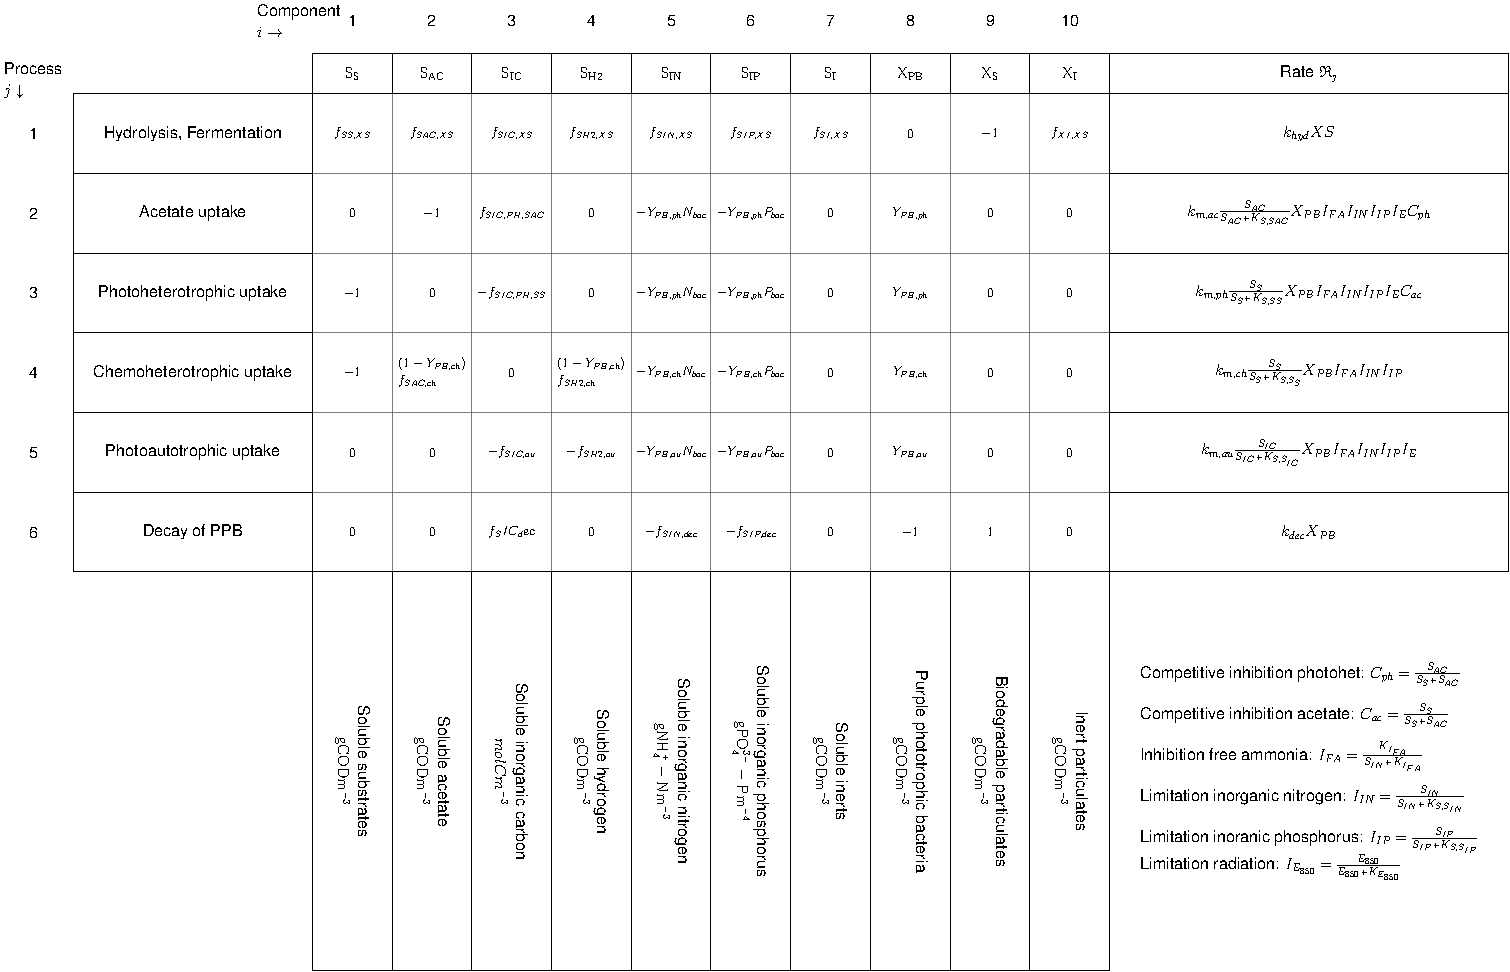
\includegraphics[width=1\linewidth]{Tables/petersen/petersen.pdf}
\end{sidewaystable}

\subsubsection{Integration with ASM models and ADM1}
Each component in the PAM-1 model can be translated into the family of IWA models. The organic compounds in this model can be transformed to ASM organic substrate by combining the acetate and other soluble organics fields. For organic particulates, $\mathrm{X_S}$ are the same for both ASM models and PAM-1. For soluble organics, $\left(S_S + S_{AC}\right)_{PAM1} \rightarrow \left(S_S\right)_{ASM}$. This quantity can then be translated to ADM1 through a model translation interface \cite{nopens2009}. Both biodegradable and inert particulates, as well as inert solubles have direct analogues in both ASM and ADM1 models. Phototrophic biomass can be converted to ADM1 via the following relationship, $X_{PB} \rightarrow \left(aX_{ch} + bX_{li} + cX_{pr} + dX_I \right)$. The coefficients $a$, $b$, $c$, and $d$ are determined through the nutrient and COD ratios of the biomass, which have been determined experimentally \cite{hulsen2014}. For inorganic nitrogen, $\left(S_{IN}\right)_{PAM\mbox{-}1} \rightarrow \left(S_{nh} + S_{no}\right)_{ASM}$. There are no changes for PAM-1 to ADM1 conversions of ammonium. To convert inorganic phosphorus, $\left(S_{IP}\right)_{PAM\mbox{-}1}$ can be expressed as either $\left(S_{IP}\right)_{ADM1}$ or $\left(S_{PO_4\mbox{-}P}\right)_{ASM2d}$. Inorganic carbon in both PAM-1 and ADM1 are expressed in the same manner, and $\left(S_{IC}\right)_{PAM\mbox{-}1}$ can be transformed into alkalinity in ASM as per the ADM/ASM model interface \cite{nopens2009}.

\subsection{Experimental procedure}
Parameters were identified through a series of batch tests. The inoculum was sourced from a 2 L photoanerobic membrane bioreactor (PAnMBR) with steady-state operation of over 300 d \cite{hulsen2016}. The inocula were different for each batch test, however the provenance and reactor operation procedure were the same across each batch test. Domestic wastewater was sourced as feed for the PAnMBR and was collected from the Taringa and St. Lucia wastewater stations (Brisbane, Australia). The average strength of wastewater over the period was 572 $\mathrm{g COD m^{-3}}$ total COD and 241 $\mathrm{g COD m^{-3}}$ of soluble COD. There were 63 $\mathrm{g N m^{-3}}$ and 9 $\mathrm{g P m^{-3}}$ for ammonium and phosphorus respectively. In tests where wastewater was not used, synthetic Ormerod medium was used as per the batch tests carried out in previous studies \cite{hulsen2014}. 
\skippingparagraph
All batch tests for metabolic growth were done in 100 mL volumes in 160 mL serum flasks. The tests were carried out in triplicate. Once the flasks were inoculated and dosed, they were flushed with $\mathrm{N_2}$ to remove oxygen from the headspace. All experiments were done at $\mathrm{20 \, \degree C}$ in an orbital shaker at 150 rpm (Edwards Instrument Company). The flasks were irradiated with 150 W lamps and the UV and visible parts of the spectrum were filtered out using photo foil as described in previous batch experiments \cite{hulsen2014}. Blank samples with zero substrate were included in all metabolic experiments.
\skippingparagraph
For hydrolysis and decay tests, the inoculum was collected in the same manner. Biomass were centrifuged in 50 mL Falcon tubes at 3750 rpm, with the pellet resuspended in 0.2 M NaCl. The centrifugation/resuspension process was done three times. The biomass was then placed in 500 mL of 0.2 M NaCl and was then redistributed into 2 250 mL Schott bottles. The bottles were flushed, placed on magnetic stirrers at 200 rpm for 30 days of operation. In order to analyse hydrolysis, aluminium foil covered one of the bottles so that no phototrophic growth would occur. Samples were taken twice-weekly for COD, VFA, $\mathrm{NH_4\mbox{-}N}$, $\mathrm{PO_4\mbox{-}P}$, total inorganic carbon (TIC), and pH. Headspace measurements were taken at the same interval for $\mathrm{CH_4}$, $\mathrm{H_2}$, $\mathrm{CO_2}$. Total suspended solids (TSS) and volatile suspended solids (VSS), as well as total Kjeldahl nitrogen (TKN) and total phosphorus (TP) were sampled and analysed every 7 days. The decay test was done with the same irradiance as that used in the metabolic growth tests. Measurements were made for TSS, VSS, TKN and TP and were taken every 7 days to monitor biomass decay. The test was done with 100 $\mathrm{g COD m^{-3}}$ of acetate and 10 $\mathrm{g N m^{-3}}$ of ammonium. 
\skippingparagraph
Specific phototrophic activities were determined by both non-linear regression, and linear regression of biomass-normalised substrate concentration within a region of maximum consumption. All conditions for batch tests are summarised in Table \ref{tab:batch}. The HEPES buffer system was dosed at 5.9 g L\textsuperscript{-1} and the phosphate buffer contained 0.9 g K\textsubscript{2}HPO\textsubscript{4} and 0.66 g KH\textsubscript{2}PO\textsubscript{4}. The carbon sources are presented in gCOD m\textsuperscript{-3} and the electron donor for photoautotrophy is presented in g m\textsuperscript{-3}. 

\begin{table}[tp]
    \centering
    \small
    \renewcommand{\arraystretch}{1.4}
    \caption{Batch conditions for metabolic tests}
    \tabcolsep=0.11cm
    \begin{tabular}{@{}p{3cm} p{1.4cm} p{1.5cm} p{1.7cm} p{1.4cm} p{1.4cm} p{1.4cm} p{1.4cm} p{1.4cm}@{}} \toprule
        Mechanism & Medium & Buffer system & COD:N:P\textsuperscript{**} & C source & Electron donor & Electron acceptor & Positive control & Negative control\\
        \hline
        Photoheterotrophy & Ormerod& HEPES & 100:10:2 & Acetate (130), propionate, butyrate, ethanol (100) & Organic & CO\textsubscript{2}&  $\mathrm{1\, g}$ NaHCO\textsubscript{3} added&  -- \\
        
        Nitrogen limitation & Ormerod&  HEPES & 100:1.4:2& Acetate (130) & Organic & CO\textsubscript{2}& No limitation & -- \\
        
        Phosphorus limitation & Ormerod & HEPES & 100:10:0.15 & Acetate (130) & Organic & CO\textsubscript{2}& No limitation & -- \\
        
        Photoautotrophy & Ormerod & Phosphate & 100:20:$\infty$ & NaHCO\textsubscript{3} (140\textsuperscript{*}) & Na\textsubscript{2}S (300)& CO\textsubscript{2}& -- & No Na\textsubscript{2}S \\
        
        Chemoheterotrophy & Ormerod & HEPES &100:10:2 & Ethanol (60), Acetate (130) & Organic& Acetate& + light& -- \\
        
        Inhibition of $\mathrm{H_2}$ production & 
        Ormerod & Phosphate & 100:15:$\infty$&Acetate (600) & Organic & CO\textsubscript{2} & --  & N limitation (1/10) \\
        ---\texttt{"}---& DWW & -- & 100:12:4 &DWW (278) & Organic & CO\textsubscript{2}&-- &Acetate (600) \\
        \bottomrule
    \end{tabular}
    \footnotesize
    \begin{tabular}{@{}p{4cm} p{10cm}}
        \textsuperscript{*}Units are gC m\textsuperscript{-3} & \textsuperscript{**} $\infty$ means excessive concentration due to buffer \\
    \end{tabular}
    \label{tab:batch}
\end{table}

\subsection{Analytical methods}
Total and soluble COD (TCOD and SCOD respectively) were determined by COD cell tests (Merck, 1.14541.0001, Darmstadt, Germany). Dissolved $\mathrm{NH_4\mbox{-}N}$ and $\mathrm{PO_4\mbox{-}P}$ were measured by a QuikChem8000 Flow Injection Analyser (FIA) (Hach Company, Loveland, USA). Temperature and pH were measured using an Oakton pH 11 Series (Vernon Hill, Illinois, USA). Determination of TSS and VSS was done by filtration. The samples were filtered with a known volume of biomass suspension, dried in an oven at 105 $\pm$ 2 $\degree$C for 24 hours and weighed for TSS. For VSS, the same sample was then placed in a furnace at 550 $\pm$ 5 $\degree$C for 2 hours \cite{americanpublichealthassociation1998}. The incident irradiance ($\mathrm{Wm^{-2}}$) was measured with an infra-red sensor (PAS Port\texttrademark, Roseville, California, USA). VFA samples were analyzed by gas chromatography (Agilent Technologies 7890A GC System, Santa Clara, California, USA) equipped with a flame ionization detector (GC/FID) and a polar capillary column (DB-FFAP). Gas samples were analyzed by GC (2014 Shimadzu, Kyoto, Japan) with thermal coupled detector \cite{tait2009}. TKN and TP were determined using sulfuric acid, potassium sulfate and copper sulfate catalyst in a block digester (Lachat BD-46, Hach Company, Loveland, CO, USA) \cite{patton1992}. TIC was analyzed by using a total organic carbon (TOC) analyzer (Shimadzu TOC-L CSH TOC Analyzer with TNM-L TN unit) coupled to a near infrared detector (NIRD) for measuring the CO2. All soluble constituents were determined after filtering with a 0.45 mm membrane filter (Millipore, Millex\textsuperscript{\textregistered}-HP, Merck Group, Darmstadt, Germany).

\subsection{Data analysis}
\subsubsection{Data handling}
The concentration of phototrophic biomass was calculated from the method for determining VSS. The biomass was then converted to a COD quantity by the molecular formula CH\textsubscript{1.8}O\textsubscript{0.38}N\textsubscript{0.18} \cite{mckinlay2010}. This gave 1.78 kg COD for 1 kg biomass as VSS. Biomass yields were calculated from initial and final biomass concentrations based on the consumption of substrate during the batch tests. The yields (in concentration of VSS) were then converted to COD and expressed as unitless quantities (kgCOD\textsubscript{PPB} kgCOD\textsuperscript{-1}). 

\subsubsection{Statistical analyses and uncertainty analysis}
When samples were measured to be outside of the range of calibration for a given test, the measurements were repeated by dilution of the samples. Internal or external standards were used for all measurements. Calibration of all measurement equipment was done at least once per week. All parameters were estimated from triplicate samples by with the minimisation of the cost function (J) chosen as residual sum of squares Eq. \eqref{eq:cost_function}.
\begin{equation}
    \label{eq:cost_function}
    \underset{\Theta}{\mathrm{min}}\, \, \mathrm{J}(\Theta)\quad  = \quad \sum_{i = 1}^{n\in\mathbb{N}} \left(y_i - \hat{y}(\Theta)_i    \right)^2
\end{equation}

\noindent where $\Theta$ is the set of parameters that must be found such that the squared distance between the experimental data points $y_i$ and the hypothesised model $\hat{y}_i$ is minimised. For multiple parameter optimisation, the value of J was set to a critical J value (J\textsubscript{crit}) based on the F statistic determined by the number of parameters of interest, the number of data points and the significance threshold (here 95\%). \cite{batstone2003}. Uncertainty in parameters was determined from their standard error and a two-tailed Student t-test (5\% threshold). All determined parameters are expressed in terms of 95\% confidence intervals. The error bars in experimental data represent 95\% confidence intervals in mean based on a two-tailed t-test. The uncertainty of the slope when determining specific phototrophic activities was done using the Microsoft Excel 2013 Regression tool and was rechecked using the Scipy Stats package \cite{jones2001}. Unless otherwise stated, all statistical analyses were done with a 5\% significance threshold.

\subsection{Simulations of PAM-1}

\subsubsection{Simulation of a phototrophic batch system}
The model was tested to explore different scenarios in order to understand the limits of the process and to highlight the possible adaptations of he model by biomass shifts on metabolism. The model was implemented using SciPy \cite{jones2001} and NumPy \cite{walt2011} for numerical functionality, and Matplotlib \cite{hunter2007} for visualisation of results. A series of three simulations were done on a PAnMBR system.
\skippingparagraph
The first simulations were designed to assess the effects of limiting substrate concentrations on the uptake of other substrates. A range of inorganic nitrogen initial concentrations (0 gN m\textsuperscript{-3} to 60 gN m\textsuperscript{-3}) and SCOD (S\textsubscript{S} + S\textsubscript{AC}) ranging from 0 gCOD m\textsuperscript{-3} to 600 gCOD m\textsuperscript{-3} (equally divided) were simulated with all other substrates in excess. The same simulation was done for inorganic phosphorus where the range of initial concentrations was from 0 gP m\textsuperscript{-3} to 125 gP m\textsuperscript{-3} and the same initial concentrations for SCOD. 
\skippingparagraph
The second simulations were designed to examine the effect of dark/light cycles on PPB metabolism under low and high rates of chemoheterotrophic activity (k\textsubscript{M,ch} = 0.074 and 0.7 d\textsuperscript{-1} respectively). The light/dark cycling were toggled for a duration of 12 hours at a time over a simulated period of two days. 
\skippingparagraph
The third simulation looked at the differences in specific photoautotrophic activities between the results in this study, and the values found in literature.



\subsubsection{Simulation of a phototrophic continuous system}
The kinetic expressions developed in this study were used in the development of a continuous PAnMBR model. The concentration of bioavailable SCOD in medium strength wastewater was insufficient for the system to achieve TN and TP discharge limits \cite{hulsen2016}. To achieve full removal, additional SCOD was required. The goals of the simulation were the following: a) to highlight the requirement of additional SCOD to achieve total nutrient removal, and b) to demonstrate that the inclusion of a primary clarifier can lead to an organic sludge enriched in PPB biomass. Dynamic influent data was simulated according to an influent generator model \cite{gernaey2011}, and adapted to the typical concentrations of primary influent previously reported \cite{hulsen2014}. Based on the average influent characteristics and an hydraulic retention time (HRT) of 12 h, volumetric loading rate (VLR) of 400 $\pm$ 12 gCOD m\textsuperscript{-3} d\textsuperscript{-1} and a solids retention time (SRT) of 3 d, a reactor volume of 70 m\textsuperscript{3} was applied. An ideal primary clarifier was included, with a solids removal efficiency of 60\% $\pm$ 3\% \cite{tchobanoglous1991}. The generation of realistic influent was done in Simulation and subsequent data processing were done in Matlab Simulink (MATLAB R2015a, The MathWorks Inc., Natick, MA) and the simulations and data processing were done using SciPy, NumPy and Matplotlib in Python 3 \cite{jones2001, walt2011, hunter2007}. The \texttt{odeint} subroutine was sufficient for solving the stiff system of differential equations. 
\skippingparagraph
The case was simulated for 609 days with 3 stages of differing SCOD concentrations (Table \ref{tab:cont}). The dynamic influent after settling was applied directly during Stage I until day 300. During Stage II (days 300-450), acetate was added to the optimum COD:N:P ratio of 100:7.1:1.8 based on the limiting nutrient (N or P). During Stage III, acetate addition was ceased. This was to assess process response to a sudden change, and to demonstrate that the system requires wastewater with a specific COD/N/P ratio. State equations were implemented in a fixed volume, completely mixed membrane bioreactor. The results from the simulation were balanced over COD, N, P and C. The simulation has been packaged into a Jupyter notebook at \textbf{Gitlab Release for PAM notebook}. For the continuous simulations, the balance equations Eq. \eqref{eq:cont} were modified to include flows, and it was assumed that a membrane would retain all particulate matter such that the solids retention time (SRT) was fixed. The explanation of variables used are summarised in Table \ref{tab:cont_op_conditions}. 

\begin{table}[tp]
    \centering
    \small
    \renewcommand{\arraystretch}{1.4}
    \caption{Continuous operating periods for the PAnMBR}
    \tabcolsep=0.11cm
    \begin{tabular}{@{}p{2cm} p{4cm} p{5cm} p{2cm}@{}} \toprule
        Phase & Condition & Value & Time (d) \\ 
        \hline
        I & DWW & 273 $\mathrm{\pm 1 \times 10^{-3}\, gCOD\, m^{-3}}$ & [150;300)\\
        II & Acetate addition & 383 $\mathrm{\pm 2 \times 10^{-3}\, gCOD\, m^{-3}}$ & [300;450)\\
        III & DWW & 260 $\mathrm{\pm 1 \times 10^{-3}\, gCOD\, m^{-3}}$ & [450;609]\\
        \bottomrule
    \end{tabular}
    \label{tab:cont}
\end{table}

\begin{align}
    V \frac{dS_i}{dt} \, &= \, Q_f (S_{fi} - S_i) + V {R}_i  \nonumber \\
    V \frac{dX_i}{dt}\, &= \, Q_f (X_{fi} - X_i) + Q_o X_i + V {R}_i
    \label{eq:cont}
\end{align}

\begin{table}[tp]
    \centering
    \small
    \renewcommand{\arraystretch}{1.4}
    \caption{Continuous operating periods for the PAnMBR}
    \tabcolsep=0.11cm
    \begin{tabular}{@{}p{7cm} p{4cm} p{5cm}@{}} \toprule
        Variable  & Value & Unit \\ 
        \hline
        V: reactor volume & $\mathrm{70}$ & $ \mathrm{m^{-3}}$ \\
        S\textsubscript{i}: concentration of soluble species i & Dynamic data & 383 $\mathrm{gCOD\, m^{-3}}$ \\
        X\textsubscript{i}: concentration of particulate species i & Dynamic data & 260 $\mathrm{gCOD\, m^{-3}}$ \\
        Q\textsubscript{f}: feed flow rate  & 14.110 $\pm$ 0.44 & $\mathrm{m^3\, d^{-1}}$\\
        S\textsubscript{fi}: feed concentration of soluble species i & Dynamic data & \{gCOD, gN, gP, mol C\} m\textsuperscript{-3}\\
        X\textsubscript{fi}: feed concentration of particulate species i & Dynamic data & gCOD m\textsuperscript{-3}: \\
        Q\textsubscript{o}: liquid flow rate out & Dynamic data&  $\mathrm{m^3\, d^{-1}}$\\
        ${R}$\textsubscript{i}: rate of reaction of species i & [-] & \{g COD, gN, gP, mol C\} m\textsuperscript{-3} d\textsuperscript{-1} \\
        \bottomrule
    \end{tabular}
    \label{tab:cont_op_conditions}
\end{table}




\newpage
\section{Results and discussion}
Inoculum for all experiments cam from a lab-scale photo-anaerobic membrane bioreactor. Most organisms are related with $\alpha$\textit{-proteobacteria}, PPB accounting for greater than 70\% of gene copies detected by pyrosequencing. \textit{Rhodobacter sphaeroides} accounts for more than 60\% of the microbiota \cite{hulsen2016}. Other photosynthetic organisms accounted for less than 1\% of the total gene copies, meaning that photosynthetic or phototrophic biomass was mostly PPB. 










%------------------------------------------------------------------------------
%                     SUPPLEMENT THIS SECTION
%------------------------------------------------------------------------------




\subsection{Growth processes}
Photoheterotrophic growth was assessed with volatile fatty acids (VFA) and ethanol. All substrates were completely consumed during the experiment, and overall yields were similar in all cases (average biomass yield of 1.13 $\pm$ 0.21 gCOD\textsubscript{biomass} gCOD\textsuperscript{-1}. Excluding acetate, the uptake rates of organic substrates were similar, with a k\textsubscript{M,ph} of 1.4 $\pm$ 0.2 d\textsuperscript{-1}. The Monod half saturation constant K\textsubscript{S,S} was undetectable throughout the experiments. The specific phototrophic uptake rate for acetate was almost twice that of the other VFAs (k\textsubscript{M,ac}2.4 $\pm$ 0.4 d\textsuperscript{-1}). The half saturation coefficient was still low but detectable (K\textsubscript{S,AC} = 20 $\pm$ 4 gCOD m\textsuperscript{-3}). This leads to an initially fast uptake of acetate, with consumption of substrate leading to a lower rate towards the end of the batch tests. 
\skippingparagraph
Chemoheterotrophic growth tests were carried out using acetate and ethanol as substrates, with the radiative source blocked by aluminium foil. PPB biomass was much less effective in dark conditions compared to light conditions where Y\textsubscript{PB,ph} was 1.0 gCOD\textsubscript{biomass} gCOD\textsuperscript{-1} and Y\textsubscript{PB,ch} was 0.5 gCOD\textsubscript{biomass} gCOD\textsuperscript{-1}. Biomass yield in dark conditions was greater than double that reported values for dark fermentation and anaerobic oxidation processes \cite{batstone2002}. It is possible that energy storage may play an important role here due to energy storage in batch operation \cite{liang2010}. Running a photobioreactor in continuous mode may produce different results depending on the radiation frequency. For example, in a system where either photobioreactor design or hydrodynamics leads to long frequency constants of light-dark irradiation, or where natural solar radiation is used, the response is likely to be similar to the batch response seen here. However in cases where incident irradiance or hydrodynamic transport is insufficient, longer dark periods may lead to the depletion of stored energy. This hypothesis requires further investigation as there is currently no supporting literature. This could mean that the model requires extension to include the accumulation of poly-P or PHA or the consideration of methanogenic processes which dominate if phototrophic bacteria cease to remove substrates.
\skippingparagraph
Analysis of photoautotrophy was done with NaHCO\textsubscript{3} as an inorganic carbon source and Na\textsubscript{2}S as an electron donor (Table \ref{tab:batch}) supplied in excess. The biomass had a yield of 36 gCOD\textsubscript{biomass} molC\textsuperscript{-1} which is comparable to the yield on acetate (31.6 gCOD\textsubscript{biomass} molC\textsuperscript{-1}). However, the maximum uptake rate k\textsubscript{M,ic} was far lower at \num{3.4E-3} $\pm$ \num{5E-4} molC gCOD\textsuperscript{-1}d\textsuperscript{-1} (compared to \num{7.5E-2} $\pm$ \num{2E-3} molC gCOD\textsuperscript{-1}d\textsuperscript{-1} on acetate). Photoautotrophy needs to be considered for when there is an excess of bicarbonate and electrons from inorganic sources in the wastewater. It is also important to consider photoautotrophy in order to close mass balances. This case is particularly relevant in light deficiency, where fermentation and anaerobic oxidation processes may become important and hence H\textsubscript{2} is available as a major electron source for PPB.
\skippingparagraph
Nutrient limitation experiments for N and P were used to determine respective half saturation coefficients. K\textsubscript{S,IN} and K\textsubscript{S,IP} values were extremely low such that N and P regulation became a switch function. Biomass assimilated nutrients at a COD:N:P ratio of 100:7.1:1.8, which is higher than conventional aerobic bacteria and much higher than other anaerobes \cite{tchobanoglous1991}. These values are in line with previous works \cite{hulsen2014}. However, PPB were able to grow at a lower rate once the nutrients were completely consumed (42\% lower than in full nutrient conditions), likely due to fixation of headspace N2 \cite{hunter2008} which would have been inhibited while ammonium was in the system. Nitrogen fixation is completely inhibited at any concentration of ammonium less than 20 gN m\textsuperscript{-3}), and nitrogenase activation requires a lag phase of low ammonium concentration in order to be reactivated, likely due to activation of the transcription of nitrogenase genes during cell maintenance conditions \cite{masepohl2002}. Additionally, PPB can accumulate polymers such as poly-P \cite{liang2010} as well as PHA \cite{melnicki2009} which can be used during cell maintenance. Since the model developed here is sustained on biomass growth in presence of ammonium, nutrient limitation for growth must be included.

\subsection{Endogenous processes}
Hydrolysis and decay are considered as transversal first order biochemical processes in most models \cite{batstone2006, henze2000, szilvester2010}. These could be considered separately, since phototrophic growth can be restricted in the absence of irradiance, and decay can be determined directly by measuring phototrophic activity following periods of irradiation without substrate. Biomass activity reduced according to first order kinetics, with a decay coefficient of \num{0.09} $\pm$ \num{0.04} d\textsuperscript{-1}. Hydrolysis was determined in dark conditions with sufficient substrate such that phototrophic biomass could not re-assimilate hydrolysis products. The products of hydrolysis (all soluble substrates included in the model) were measured and correlated with the first order kinetics of the hydrolytic process. The hydrolysis coefficient was \num{0.07} $\pm$ \num{0.004} d\textsuperscript{-1}. Hydrolysis is substrate specific, and depends highly on operating conditions \cite{batstone2015}, but the determined value was comparable with those for anaerobic conditions, but much lower than for anaerobic processes \cite{henze2000}. 

\begin{table}[tp]
    \centering
    \small
    \renewcommand{\arraystretch}{1.4}
    \caption{Summary of estimated parameters and comparison to literature values}
    \tabcolsep=0.11cm
    \begin{tabular}{@{}p{2cm} p{3cm} p{4cm} p{4cm} p{3cm} @{}} \toprule
        Parameter & Units & Value & Literature value & Source \\
        \hline
        k\textsubscript{M,ac} & d\textsuperscript{-1} &2.4 $\pm$ \num{0.4}  & 1.5 $\pm$ \num{0.5}  &\cite{golomysova2010, mckinlay2011}\\
        
        k\textsubscript{M,ph} & d\textsuperscript{-1} &1.4 $\pm$ \num{0.2}&11 $\pm$ 13 & \cite{golomysova2010, gadhamshetty2008, klein1991, mckinlay2011, obeid2009}\\
        
        k\textsubscript{M,ch} & d\textsuperscript{-1} &\num{7.4E-02} $\pm$ \num{4E-3}&5 $\pm$ 4& \cite{madigan1978, schultz1982}\\
        
        k\textsubscript{M,ic} & molC gCOD\textsuperscript{-1} d\textsuperscript{-1} &\num{3.4E-03} $\pm$ \num{5E-4} &\num{0.025} $\pm$ \num{0.018} &  \cite{sarles1983, wang1993}\\
        
        k\textsubscript{hyd} & d\textsuperscript{-1} & \num{7.1E-02} $\pm$ \num{0.005}& \num{0.27} $\pm$ \num{0.06} & \cite{huangju-sheng1999, huang2001}\\
        
        k\textsubscript{dec} & d\textsuperscript{-1} & \num{9.0E-02} $\pm$ \num{4E-02}& \num{0.2} $\pm$ 0.02&  \cite{huangju-sheng1999, huang2001}\\
        \hline
        K\textsubscript{S,S} & gCOD m\textsuperscript{-3} & \num{0.5} $\pm$ \num{0.2} & \num{4e3} $\pm$ \num{6e3}& \cite{gadhamshetty2008,obeid2009}\\
        K\textsubscript{S,AC} & gCOD m\textsuperscript{-3} & \num{20} $\pm$ \num{20} & [-] &[-] \\
        K\textsubscript{S,IC} & gCOD m\textsuperscript{-3} & \num{.42} $\pm$  \num{.42} & [-] &[-] \\
        K\textsubscript{S,IN} & gN m\textsuperscript{-3} &\num{0.02} $\pm$ \num{0.1} & [-]&[-] \\
        K\textsubscript{S,IP} & gP m\textsuperscript{-3} &\num{0.081} $\pm$ \num{0.01} &[-] &[-] \\
        K\textsubscript{S,E} & W m\textsuperscript{-2} & [-] & \num{8.76} & \cite{eltsova2016} \\
        \hline
        Y\textsubscript{PB,ph} &[-] & 1.0 & \num{0.78} $\pm$ \num{0.37}& \cite{gadhamshetty2008, klamt2002, klein1991, mckinlay2011, obeid2009, schultz1982} \\
        Y\textsubscript{PH,ch} &[-] & \num{0.5} &\num{0.23} $\pm$ \num{0.12} &  \cite{madigan1978, schultz1982}\\
        Y\textsubscript{PB,au} &gCOD molC\textsuperscript{-1} &36 & 130 $\pm$ 80 & \cite{wang1993} \\
        \bottomrule
    \end{tabular}
    \label{tab:bioparams}
\end{table}

\textbf{Section on the comparison of paramters}

\subsection{Batch simulations}

\subsubsection{Limiting N, P and SCOD}
In this scenario, the main metabolic pathway analysed was photoheterotrophy. Since one of the major the major of PPB biotechnology is complete assimilation of COD, N and P, it is necessary to explore the limits of the process for optimum COD:N:P ratios. These simulations were done for a domestic wastewater context.
\skippingparagraph
Fig. \ref{fig:ch2_cnp} shows the results of the simulations. The x-axis represents the concentrations of SCOD for each simulation. The y-axis in a) shows the range of concentrations of s\textsubscript{IN} and the y-axis in b) shows the varying concentrations of S\textsubscript{IP}. For both simulations, the optimal operating line for initial concentrations is shown (COD:N = 100:8.6 and 100:1.5 for figures a) and b) respectively). There are three possible regions outside the optimum according to the results shown in Fig. \ref{fig:ch2_cnp}: (i) now nutrient concentration where there is a net accumulation of SCOD in the system, (ii) high nutrient concentration where all SCOD is consumed but the effluent still contains nutrients, and (iii) insufficient COD for the maintenance of biomass growth despite the nutrients concentration and \textit{vice-versa}. Region (iii) is the only one which can not be sustained in a long-term growth process due to biomass decay. Region (i) (below the solid line), is not possible in a domestic wastewater context, where nutrients are always in excess. The most typical case is region (ii) (above the solid line), where the addition of external SCOD is necessary for the system to assimilate nutrients. This study could serve as a guide for estimating requirements in real industrial cases.  



\begin{figure}[tp]
    \hspace*{-2cm} 
    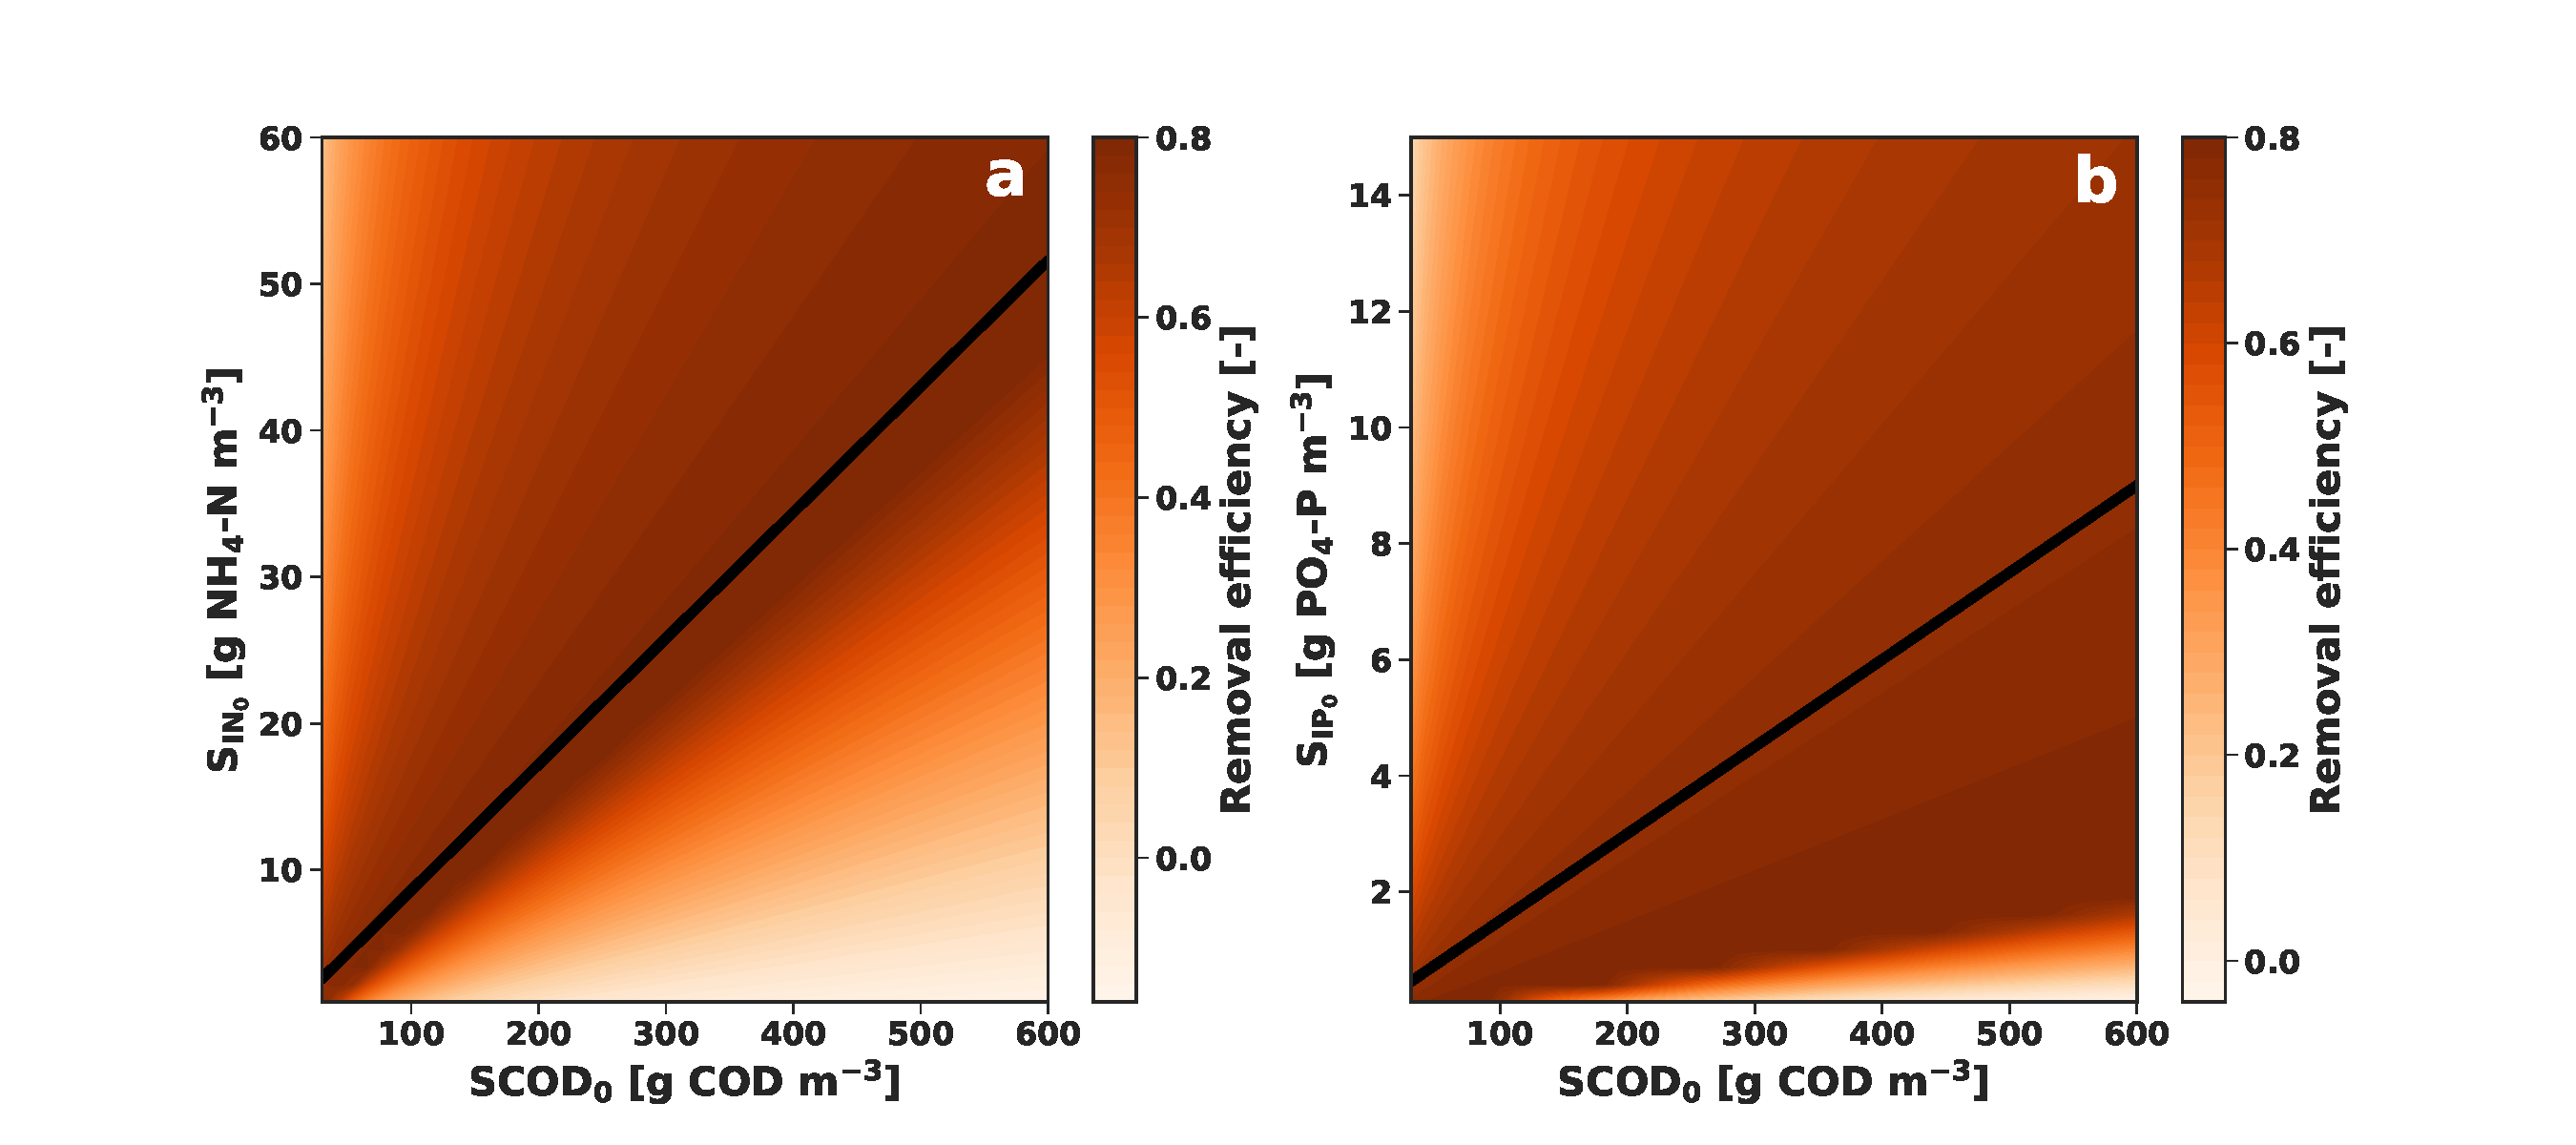
\includegraphics[width=1.25\linewidth]{./Chap2/simulations/ch2_sin_cod.pdf}
    \caption{Normalised removal efficiencies of SCOD and $\mathrm{NH_4\mbox{-}N}$ (a) and $\mathrm{PO_4\mbox{-}P}$ (b). All initial conditions were maintained constant and the initial conditions of SCOD and the respective nutrients were varied between low (close to zero) and high values (600 gCOD m\textsuperscript{-3} for SCOD, 60 gNH\textsubscript{4}-N m\textsuperscript{-3} for S\textsubscript{IN} and 15 gPO\textsubscript{4}-P m\textsuperscript{-3} for S\textsubscript{IP}).}
    \label{fig:ch2_cnp}
\end{figure}


\subsubsection{Light-dark cycling}
The parameters calculated in this work are a condition of the origin of the biomass. The PAnMBR was operated with irradiance in excess and no light-dark cycling (outside of the hydrodynamics). Although this is operation is normal for indoor photobioreactors, other configurations using solar radiation as a direct light source need consideration of the effects of light-dark cycling on biomass growth. During the night, phototrophic biomass in outdoor photobioreactors need to make use of an energy source other than radiation. Therefore it is clear that the metabolism would shift to chemoheterotrophic growth. Several authors have found that PPB are able to follow chemoheterotrophic metabolism achieving substrate uptake rates at least one order of magnitude higher than those calculated in this work (see Table \ref{tab:bioparams}). It is therefore necessary to explore how the system behaves under a promoted chemoheterotrophy during light/dark cycles.
\skippingparagraph
A set of two simulations were performed by including light/dark cycles (12 hours light, 12 hours dark for at total of 2 days) for a typical batch scenario where all the conditions were fixed but the chemoheterotrophic uptake rate was modified using two different values (k\textsubscript{M,ch} = 0.074 and 0.7 d\textsuperscript{-1}). The results of the simulations can be seen in Fig. \ref{fig:ch2_kmch}.  When the biomass has a high chemoheterotrophic activity, soluble substrate is consumed giving rise to acetate accumulation that is eventually consumed during the irradiated phase of the cycle. A net production of hydrogen happens due to fermentation or anaerobic oxidation processes which can be used for promoting autotrophic growth. There can also be connotations on the possible biomass shift to autotrophic metabolism. Since the biomass yield is lower during chemoheterotrophic metabolism, there is a lower net increase of biomass. 

\begin{figure}[tp]
    \centering
    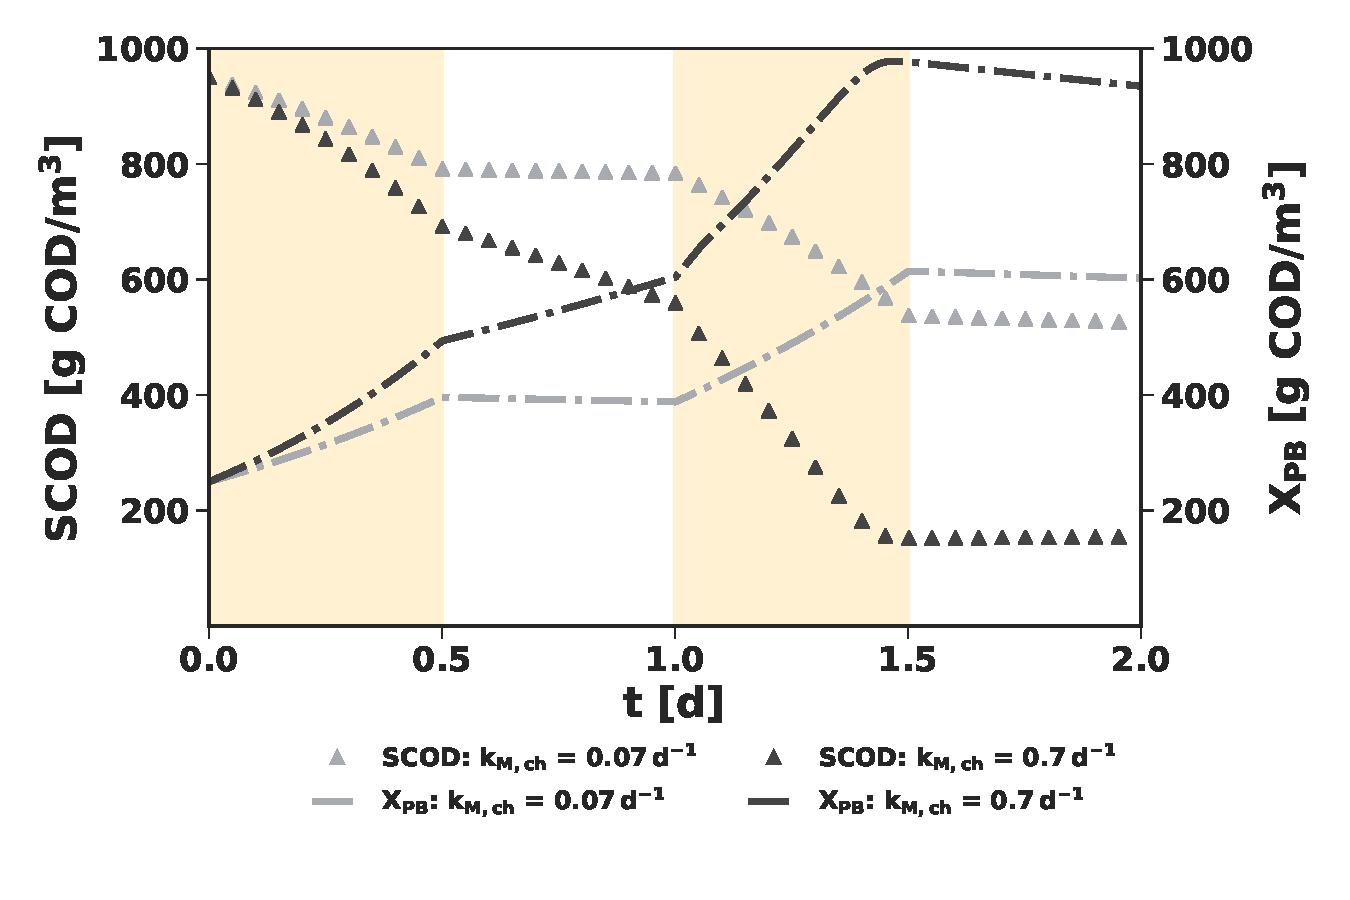
\includegraphics[width=1\linewidth]{./Chap2/simulations/ch2_kmch.pdf}
    \caption{Effect of dark/light cycling on PPB metabolism under low (light colour) and high (dark colour) chemoheterotrophic activity. There is an order of magnitude difference between the activities. A full light/dark cycle is a 24 hour period to mimic perceived solar irradiance in an outdoor photobioreactor.}
    \label{fig:ch2_kmch}
\end{figure}

\subsubsection{Sensitivity of specific photoautotrophic uptake activity}
In this scenario the promotion of autotrophy is discussed and the autotrophic metabolism is analysed. The DWW used for the batch experiments and continuous PAnMBR operation came from collection wells in Brisbane, Australia. Water in this location can be considered as moderately hard (hardness = 148 $\pm$ 7 mg CaCO\textsubscript{3} L\textsuperscript{-1}, n=19, which corresponds to 53 mgC L\textsuperscript{-1}). Therefore, there is a clear potential to enrich PPB in autotrophic conditions. However, this is only possible if there is an electron donor such as Fe\textsuperscript{2+}, S\textsuperscript{2-}, H\textsubscript{2} or reduced organics \cite{mckinlay2011}. The promotion of reductive processes such as fermentation or anaerobic oxidation (including sulfate reduction) could give rise to the reduced components for CO\textsubscript{2} fixation to be feasible. This analysis is focused on the results after the appearance of reduced conditions, and the discussion on how these conditions are possible is out of the study's scope. 
\skippingparagraph
The initial conditions of this simulation have been fixed and only the concentration of H\textsubscript{2} has been increased to 175 gCOD m\textsuperscript{-3} to cope with the stoichiometric requirements of autotrophic carbon dioxide fixation. The simulations were performed using the autotrophic uptake rate calculated here (k\textsubscript{M,ic} = $\mathrm{3.4\times10^{-6}}$ molC gCOD\textsuperscript{-1}d\textsuperscript{-1}) and a Gaussian-random set of 1000 simulations using the average literature value and 95\% confidence intervals for k\textsubscript{M,ic} (shown in Table \ref{tab:bioparams}). The simulation conditions and code is included in \textbf{Abstract 2}. The results are depicted in Fig. \ref{fig:ch2_auto}. As can be seen, the autotrophic process using calculated values seems to be residual compared to photoheterotrophic metabolism, however, photoautotrophy can be a considerable component of PPB growth. By using the mean value of k\textsubscript{M,ic} from Table \ref{tab:bioparams}, the biomass is able to fix 1 g L\textsuperscript{-1} of total inorganic carbon at the same time as they assimilate 1.76 gC L\textsuperscript{-1} through photoheterotrophic metabolism. Therefore, carbon dioxide fixation  could become a major process, which could potentially account for around 36\% of N and P removal. 


\begin{figure}[tp]
    \centering
    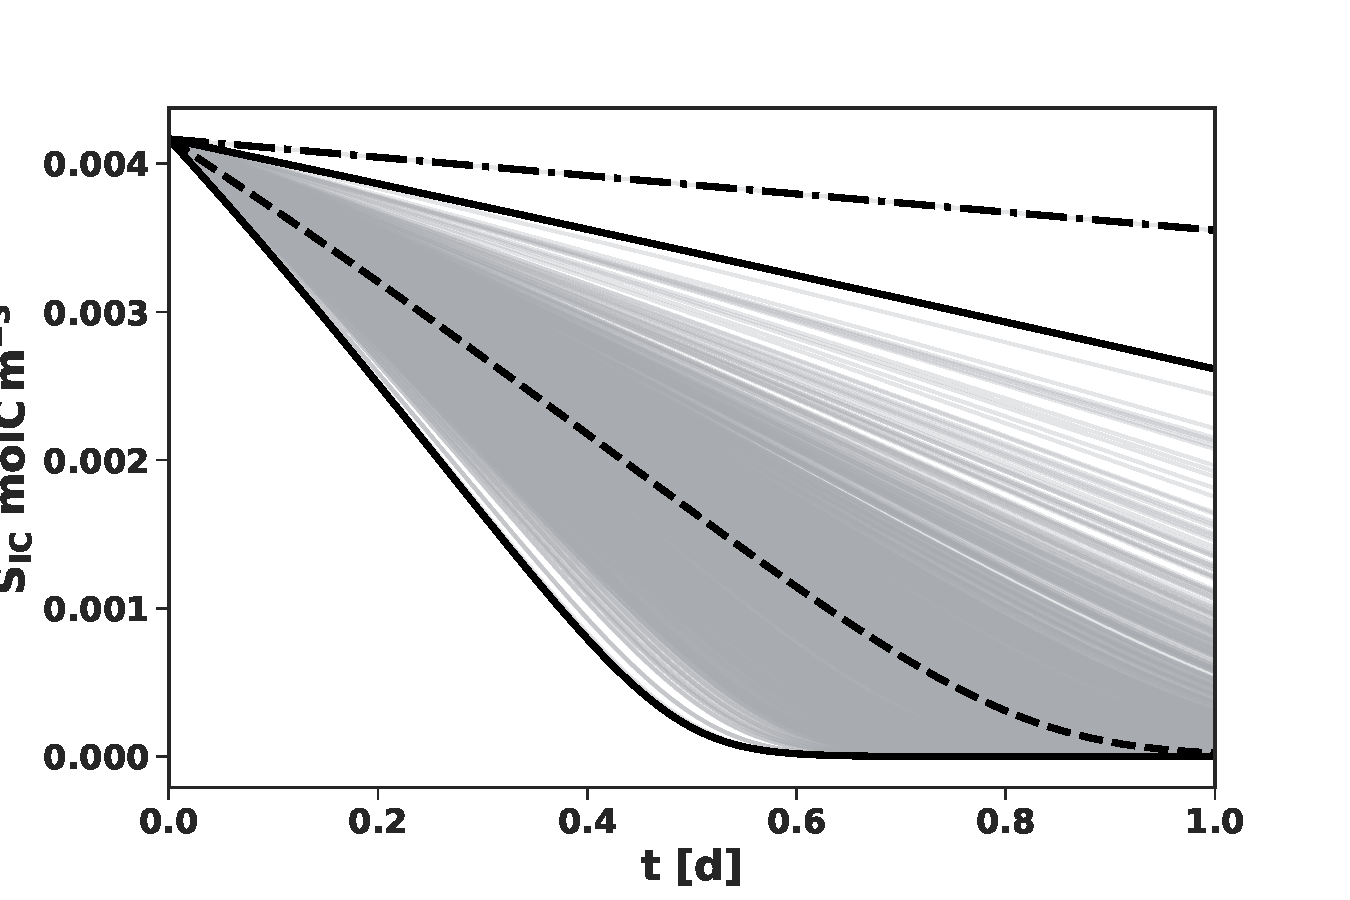
\includegraphics[width=1\linewidth]{./Chap2/simulations/ch2_auto.pdf}
    \caption{Metabolic behaviour promoted by photoautotrophy. The dashed line represents the mean literature value found for photoautotrophic uptake ($\mathrm{2.5 \times 10^{-2}}$ molC gCOD\textsuperscript{-1}d\textsuperscript{-1}). The two solid lines represent the minimum and maximum values used for the simulations from the Gaussian-random set of parameter values ($\mathrm{8.1 \times 10^{-3}}$ molC gCOD\textsuperscript{-1}d\textsuperscript{-1} and $\mathrm{4.2 \times 10^{-1}}$ molC gCOD\textsuperscript{-1}d\textsuperscript{-1} respectively). The determined value from the batch experiments was $\mathrm{3.4 \times 10^{-3}}$ molC gCOD\textsuperscript{-1}d\textsuperscript{-1} (dot-dashed line).}
    \label{fig:ch2_auto}
\end{figure}

\subsection{Continuous simulations}
\subsubsection{Fate of C, N and P}
The model indicates different SCOD removal efficiencies for particular periods of operation (Fig. \ref{fig:ch2_dyn_sol} and \ref{fig:ch2_dyn_bio}). In general, adaptation to seasonal periods of variable wastewater composition is rapid, as can be shown in input values from Figs. 5 and 6. For periods (I) and (III), which correspond to no additional acetate in the system (average inlet SCOD of 293.1 ± 0.8 gCOD L\textsuperscript{-3}), the mean SCOD removal efficiency is 81\% (Fig. 5a) The remaining SCOD in the system can be mainly attributed to the presence of non-biodegradable SCOD, accounting for 71\% of the effluent SCOD. During period (II), acetate was added to align with the COD:N:P ratio required for full nutrient and organic uptake. Average SCOD removal efficiency slightly increased to 85\% due to the optimised feed conditions. As in period (I), the major part of remaining SCOD was soluble inerts (S\textsubscript{I}). The model, however, is unable to reproduce the PPB behaviour under a high excess of inlet SCOD concentrations since it is based on assimilative mechanisms only and accumulation processes are not included. PPB biomass is able to accumulate compounds such as glycogen or polyhydroxyalkanoates \cite{melnicki2009}, so the SCOD removal efficiencies are expected to be higher and less dependent on nutrients in real cases \cite{hulsen2016,hulsen2016a}. An upgraded model including accumulative mechanisms is therefore needed for feed streams with high COD:N ratios. This model is nonetheless suitable for domestic wastewater treatment operation where N and P are usually in excess. 
\skippingparagraph
Nutrient assimilation was directly linked with biomass growth. The optimum assimilative COD/N/P relationship has been calculated to be 100/7.1/1.8 from batch experiments. Therefore, periods with non-optimal ratios are expected to have higher effluent nutrient concentrations. Under normal situation (periods (I) and (III)), with no additional acetate, nutrients were not completely removed and ammonium and phosphate efficiencies were 45\% and 56\%, respectively (Fig. 5b and c, respectively), averaging effluent concentrations of 23 gN m \textsuperscript{-1} and 2.5 gP m\textsuperscript{-3}, respectively. This justifies the need for extra SCOD addition, as has been previously described experimentally \cite{hulsen2016}. Phosphorus was almost completely removed during C and N sufficiency during period (II), with removal efficiencies of 89\% (effluent concentrations of 0.5 gP m\textsuperscript{-3}). However, depletion of P preven:ted a high N removal due to nutrient imbalance, and so N removal efficiencies during these periods averaged 70\%, averaging effluent concentrations of 11 gN m\textsuperscript{-3}. Again, accumulative mechanisms may have a key role here, as PPB are able to accumulate poly-P (Liang et al., 2010). This mechanism is quite complex and has not been properly defined, particularly in mixed cultures and on wastewater sources.
\skippingparagraph
Production of biomass was related to PPB growth as well as input solids. Biomass fractionation (X\textsubscript{PB}, X\textsubscript{S} and X\textsubscript{I}) along the simulation period is depicted in Fig. \ref{fig:ch2_dyn_bio}. When acetate was not added, PPB biomass was produced at 26.9\% of the total biomass in the outlet (sludge line). Adding acetate increased this value up to 34.9\% of total biomass. Accumulation of X\textsubscript{S} within the reactor is a direct consequence of low hydrolysis coefficient in combination with short SRT. Additional substrate increased biomass concentration due to assimilation of the remaining N and P. This also boosted the SRT, and decay was more prominent, increasing XS concentrations up to values above 1000 gCOD m\textsuperscript{-3} (see stage (II) in Fig. 6). However the fraction of inerts, was always below 32\% of the total particulates concentration, probably due to the slow hydrolysis rate. These results have an important effect on energy distribution in the PRR platform since all energy balances are directly related with the biomass management through anaerobic digestion, and the relative amount of PPB will influence potential anaerobic degradability and biomass consistency. An important aspect identified by this continuous analysis is that the biomass fraction XPB is always relatively small, even when applying a settler (compared with activated sludge streams predicted by the ASM1). This is because the hydrolysis coefficient is very low (<0.1 d\textsuperscript{1}) compared with the levels of >2 d\textsuperscript{-1} typically applied in the ASM1, ASM2 and ASM2d \cite{henze1987} (Henze et al., 2000). This means that while growth rates are comparable to activated sludge, hydrolysis rates are far lower, and hence metabolic activity is dominated by available soluble substrate (and possibly N and P) rather than electron acceptor availability. In any case, there will always be a large proportion of non-degraded particulates, due to the slow hydrolysis coefficient, and in a stable, solids dominated system, PPB sludge should be more analogous to primary sludge rather than activated sludge, with both negative and positive consequences.
\skippingparagraph
Simulation of biomass behavior has implications on biomass production upon main line biological treatment. There is a net increment of biomass production yield compared to typical activated sludge processes. This could have an impact in energy recovery (through biogas) but also in sludge waste disposal expenses, which can be partially counteracted by downstream production of high value-added bioresources as proteins, prebiotics and probiotics \cite{matassa2015} or bioplastics (Padovani et al., 2016), as well as energetic resources as third generation liquid biofuels \cite{castro2017}(Castro et al., 2016).


\begin{figure}[tp]
    \centering
    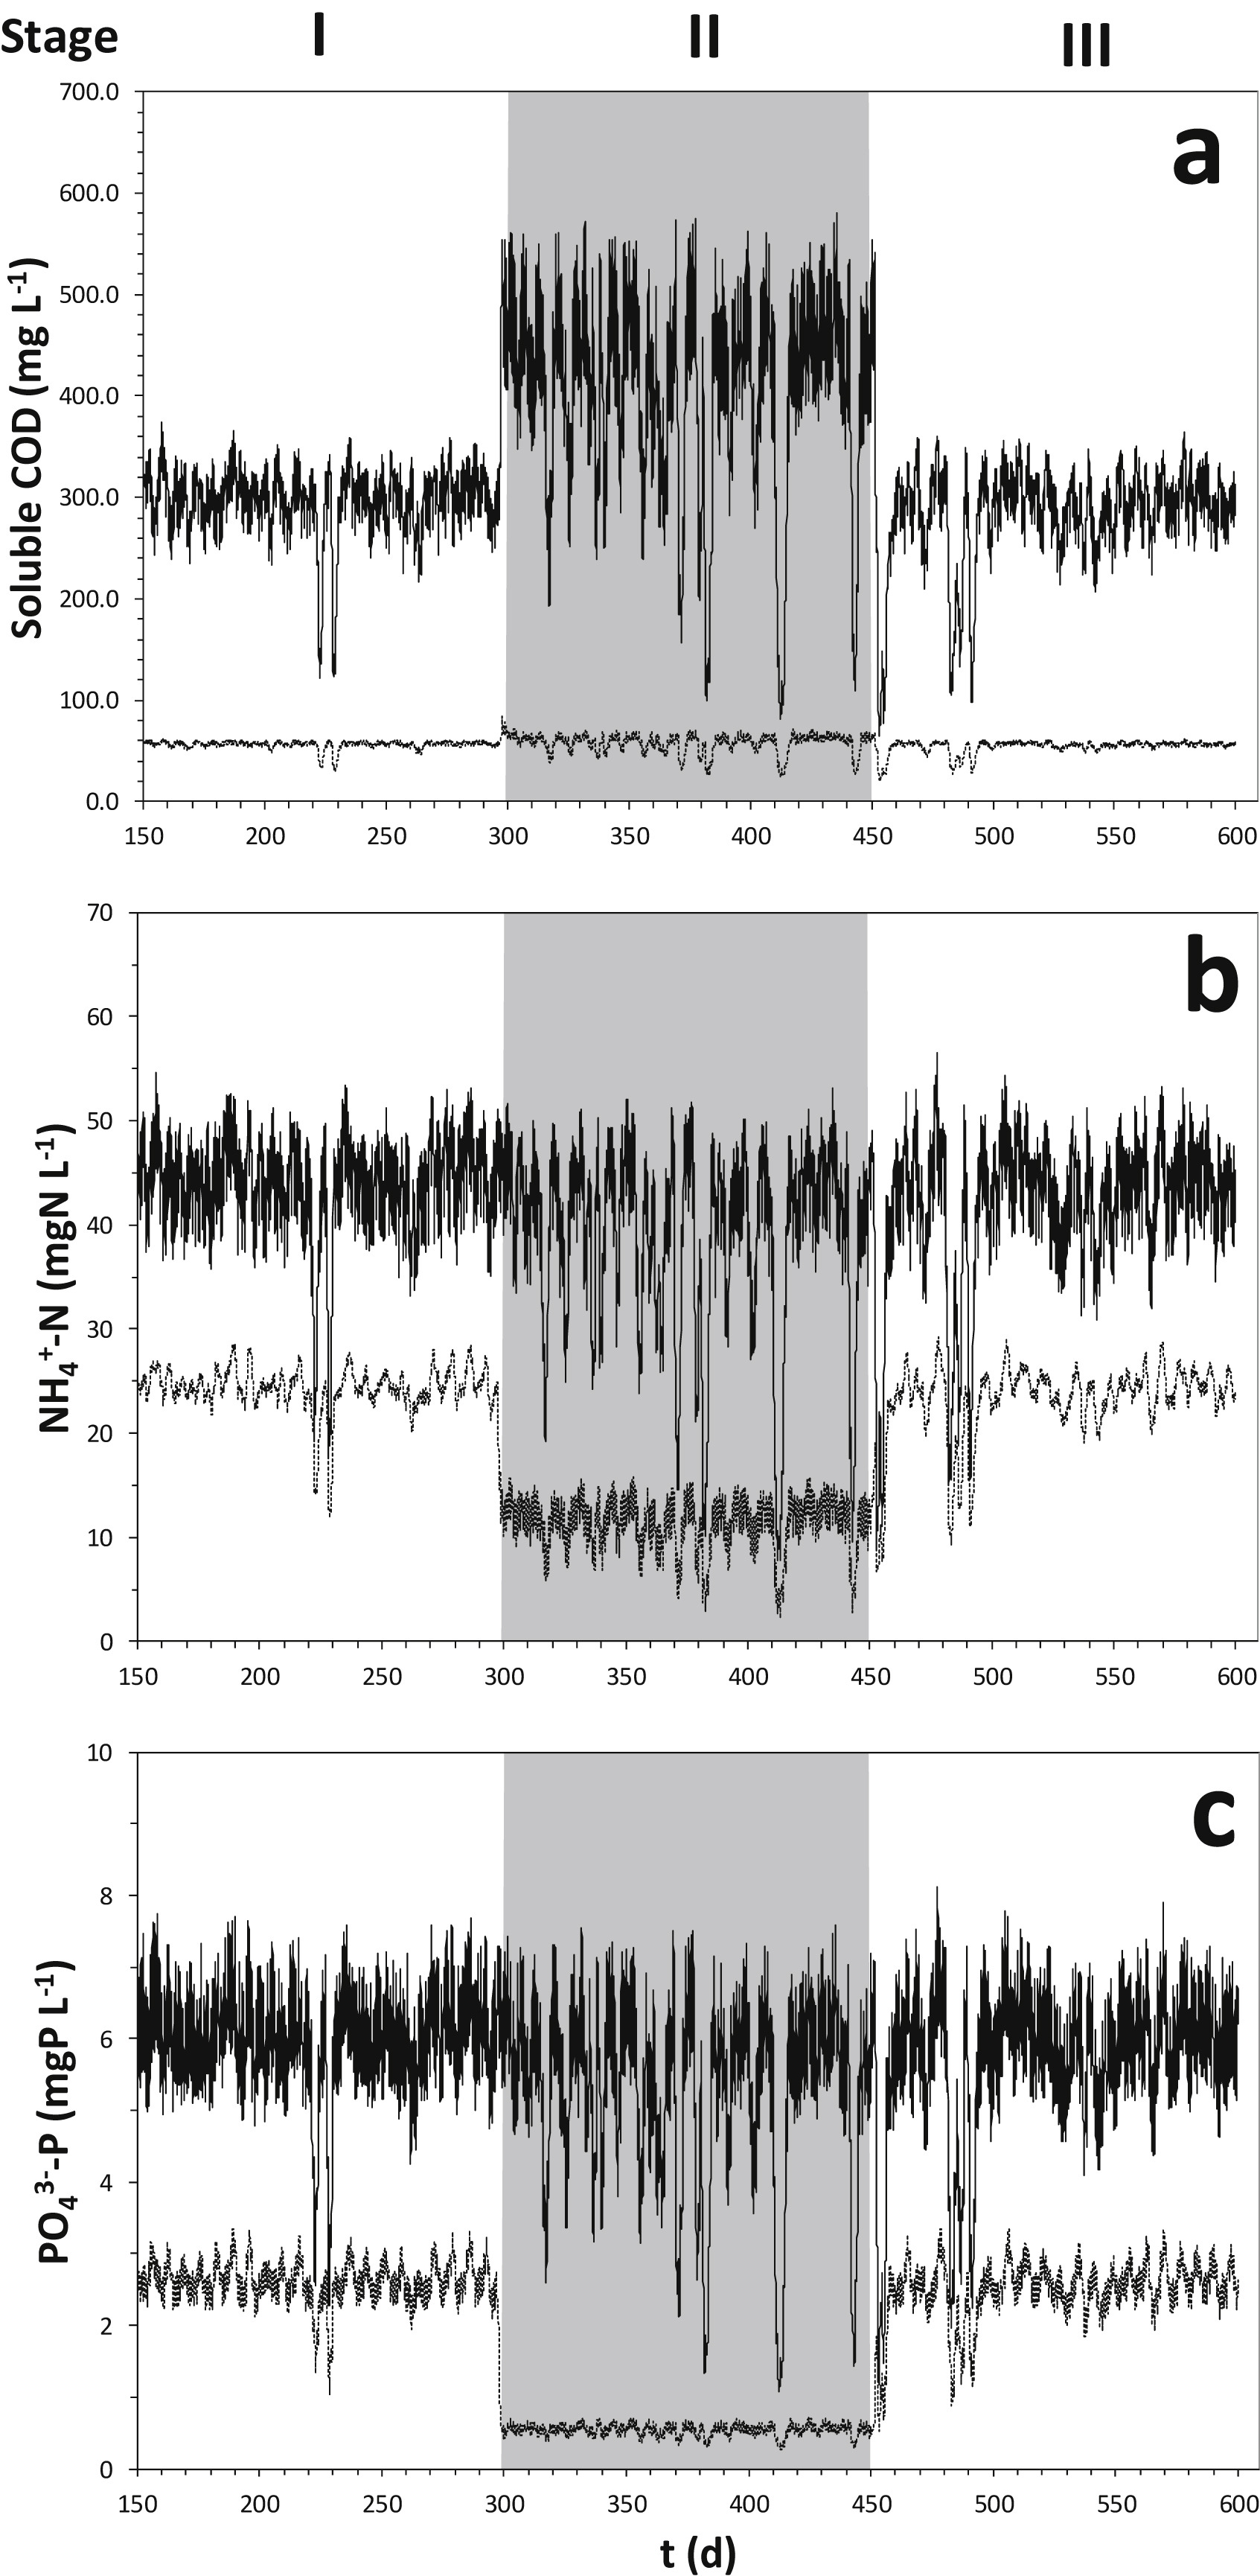
\includegraphics[width=1\linewidth,height=0.9\textheight,keepaspectratio]{./Chap2/simulations/dynamic_output.jpg}
    \caption{Influent (continuous line) and effluent concentrations (dashed line) over time for PAnMBR simulations for SCOD (a), ammonium (b) and phosphate (c) after primary settling. The different operational periods are separated by vertical shading.}
    \label{fig:ch2_dyn_sol}
\end{figure}

\begin{figure}[tp]
    \centering
    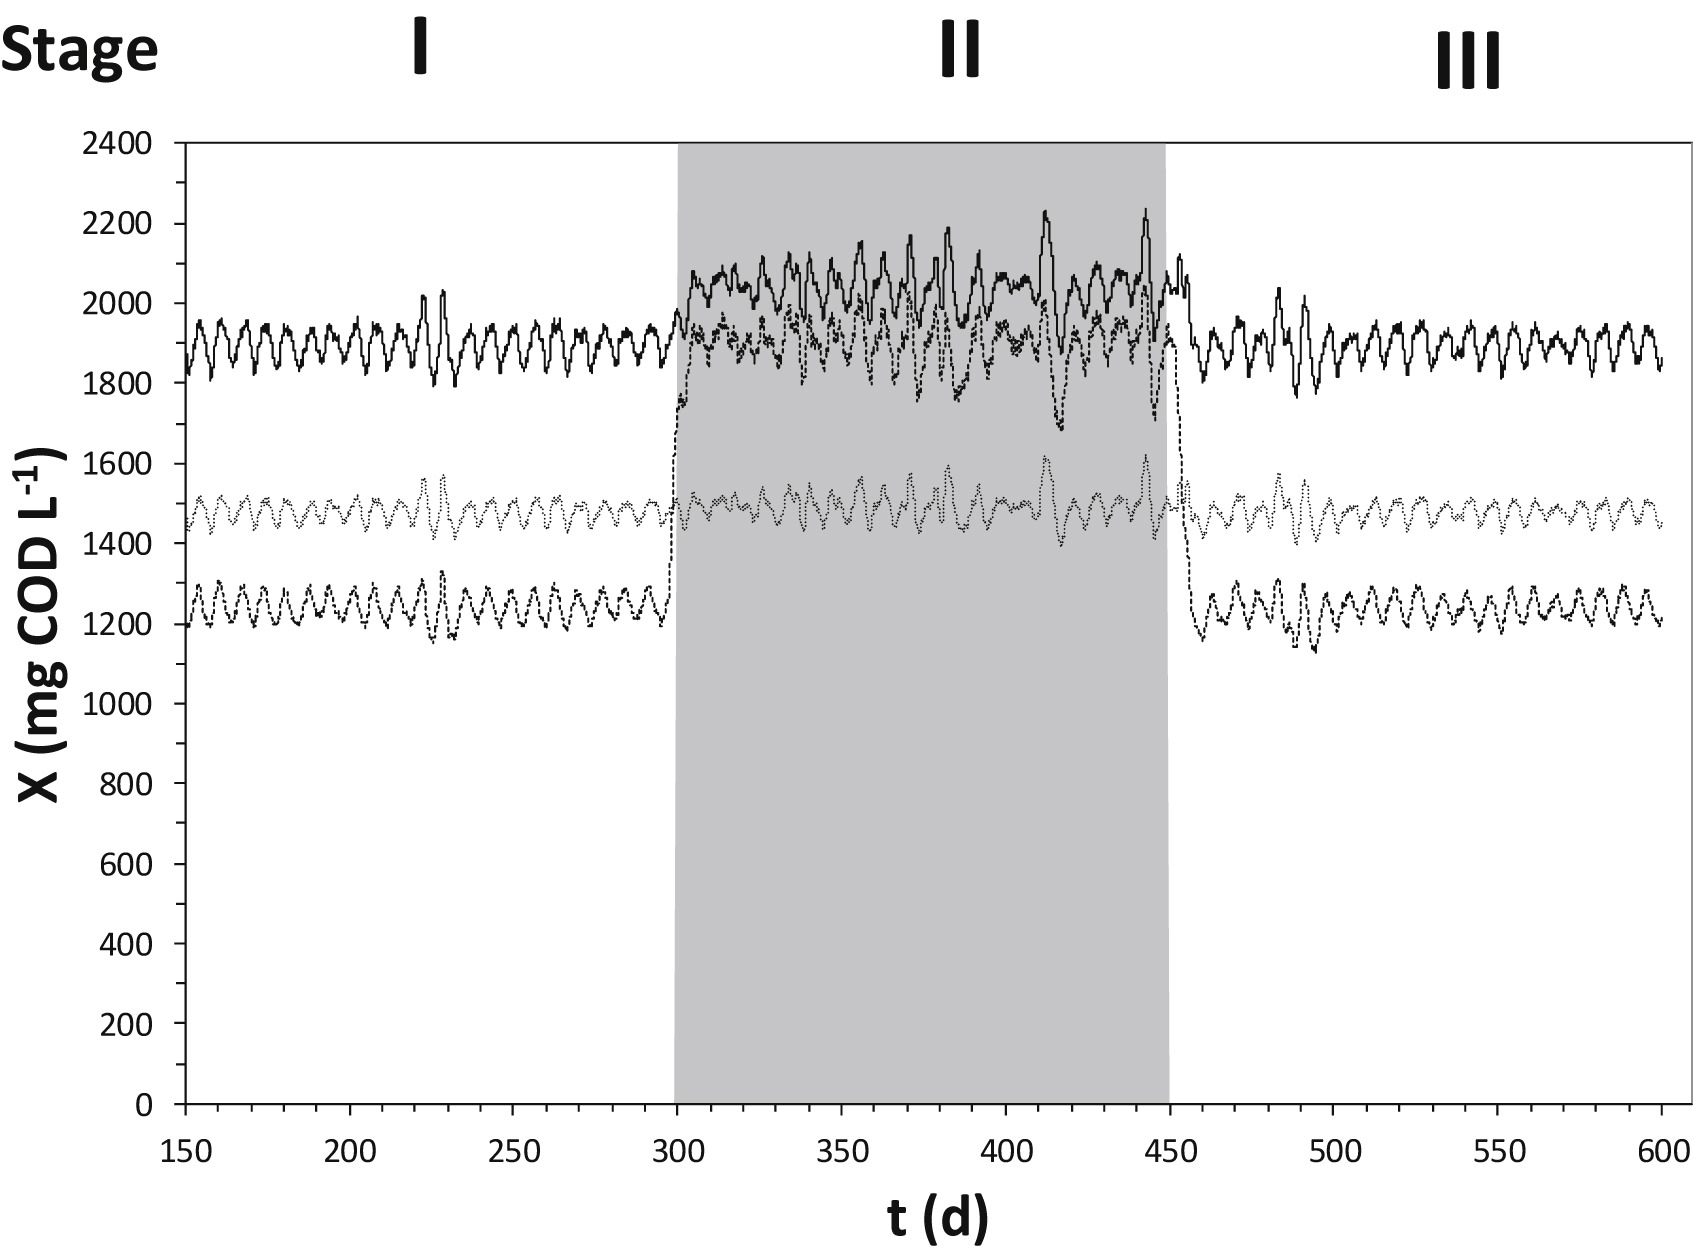
\includegraphics[width=1\linewidth,height=\textheight,keepaspectratio]{./Chap2/simulations/dynamic_biomass.jpg}
    \caption{Biomass fractionation including active phototrophic bacteria (dashed line), biodegradable particulate biomass (continuous line) and inert particulates (dotted lines) over time for the PAnMBR continuous simulation. Different operational periods are separated by differently shaded regions.}
    \label{fig:ch2_dyn_bio}
\end{figure}

\section{Conclusions}
This study presents the first model for medium strength wastewater treatment by PPB.
Anaerobic phototrophic growth in domestic wastewater treatment is fast when comparing specific uptake rates and apparent half saturation coefficients (K\textsubscript{S}) in activated sludge processes. However, hydrolysis is relatively slow, in the order of 0.1 d\textsuperscript{-1}, which means that particulate substrates will not be degraded at short hydraulic retention times. The predominant mechanism is photoheterotrophic metabolism, with both autotrophic and chemoheterotrophic growth generally slow in a wastewater treatment context. Batch simulations using different feed characteristics showed that the predominant mode of growth can shift, as is the case of high H\textsubscript{2} concentrations and their effect on photoautotrophic uptake. The decay rate is high in comparison to activated sludge under aerobic conditions. The dynamics under continuous operation conditions indicate that the biological processes are adaptable to normal flow variations such that the performance at a given mode of growth is stable. 

The following limitations of the model have been identified:
\begin{enumerate}
    \item The model is only valid for anaerobic conditions, and hydrogen production for redox balancing is assumed to be inhibited. This model therefore cannot be implemented for hydrogen production systems in its current state.
    \item Poly-P and the accumulation of other polymers is not included due to the lack of supporting literature. Nitrogen fixation has also not been included as it is assumed to be limited by ammonium.
    \item The model presents and includes biological mechanisms only. As a radiative field varies in spatial dimensions, the model should be extended to include scope to simulate spatial variations. For example, computational fluid dynamics could be used to capture the flow field and radiation characteristics, and their coupling to biomass growth. 
\end{enumerate}


A key priority for future research should be inclusion of poly-P and PHA accumulation as well as N2 fixation and side H2 production, as these processes (poly-P without carbon, PHA without oxidation or organics, and N2/H2 production) are unique to photoanaerobic organisms. The topic of infrared light delivery has not been addressed in detail in this model, and is generally assumed to be in excess (i.e., not limiting catabolic rate, such that there is no mixed photo-dark fermentation (mixotrophic growth). This could be incorporated by limiting light to enable mixotrophic growth through the existing switch function that considers also spatial separation to dark zones, but as stated above, further work is required to consider accumulation and depletion of storage compounds. This requires a very different approach to (for example, Algae) (reviewed in Béchet et al., 2013) where a more complex model is commonly applied: (considering separately excited, resting, inhibited differential states). We have kept PPB biomass as a single state, with different processes acting on it, which are in turn linked to the presence or absence of irradiance, which would enable more simple extension to energy storage and depletion. This would enable more precise determination of the switch between stored dark heterotrophic growth and methanogenesis.
%\begin{instructional}
%Add your text here. Use \verb|\cite| to add citation labels. Reference sections, tables, and figures using \verb|\ref|. Use %\verb|\eqref| for equations. The `section' symbol $\S$ is obtained using \verb|$\S$|. Figures and other floats are added using their %respective environments. Use \verb|\longtable| to split tables over page.
%\end{instructional}
